\documentclass{article}

\usepackage{fullpage}
\usepackage{graphics}
\usepackage{amsmath}
\usepackage{indentfirst}
\usepackage{setspace}
\usepackage[]{algorithm2e}
\usepackage{graphicx}
\usepackage{float}
\usepackage{xfrac}
\usepackage{xcolor}

\graphicspath{ {images/} }

\DeclareMathOperator{\var}{var}
\DeclareMathOperator{\cov}{cov}
\newcommand{\bm}[1]{\mbox{\boldmath $ #1 $}}
\newcommand{\EE}{\mathrm{I\!E\!}}
\newcommand{\RR}{\mathrm{I\!R\!}}
\parindent=0in

\doublespacing
\pagenumbering{arabic}

\begin{document}

\title{Generalised Pareto Distribution with Metropolis-Hastings MCMC updates}
\author{John O'Sullivan}
\maketitle

\section*{Introduction} \label{sec3:appenda} %\nameref{test:appenda}
\addcontentsline{toc}{section}{Appendix A}%
\markright{Appendix A}
This document includes details on the model fitted by this code; namely, it describes in detail how we modelled a dataset of extreme observations using a generalised Pareto distribution and Metropolis-Hastings Markov chain Monte Carlo updates. Details for the Binomial component of the model are similar, and are omitted here for brevity.
\\

The following pages include:
\begin{itemize}
\itemsep-0.4em
\item the pseudocode in order to programme the algorithm;
\item the model directed acyclic graph (DAG);
\item details of the model notation;
\item and the details of all equations needed for the MCMC updates of the parameters and the hyperparameters.
\end{itemize}

\subsection*{Algorithm details}

%(Filled in below):

\RestyleAlgo{ruled}
\begin{algorithm*}[H]
\BlankLine
 \KwData{$z_k(x_i)$, the declustered threshold excesses at locations $x_i, i = 1 \dots n$, with $k = 1 \dots n_i$ excesses at location $i$\;
 	$X_\phi$, $X_\xi$, $n \times (p + 1)$ and $n \times (q + 1)$ matrices of $p$ and $q$ covariates at locations $i = 1 \dots n$.}
\BlankLine
 \KwResult{Samples from the posterior distributions of $\phi=\log(\sigma)$ and $\xi$ (the unknown parameters of interest), which can then be used to calculate return level estimates and other desired quantities}
\BlankLine
 \textbf{Initialisation\;}
	Random starting values of $\phi$ and $\xi$ \;
	
 	Hyperparameter values of $\alpha_\phi$, $\beta_\phi$, $\varsigma^2_\phi$, $\tau^2_\phi$, $\alpha_\xi$, $\beta_\xi$, $\varsigma^2_\xi$, and $\tau^2_\xi$;
 	
	Number of iterations $N$\;
\BlankLine
\For{iterations $j$ from 1 to $N$}{
	Generate $u \sim U(0, 1)$\;
	\For{grid locations $i$ from 1 to $n$}{
		Simulate $\phi_{new,i}$\;
		
		Set $l_{new}$ = log full conditional of new vector $\phi_{new}$\;
		Set $l_{old}$ = log full conditional of old vector $\phi$\;
		Set $a = \exp(l_{new} - l_{old} )$, that is, evaluate equation~(\ref{3eq:1a})\;
		
		\If{$a > u$}{
			Set $\phi = \phi_{new}$\;
		}

		Simulate $\xi_{new,i}$\;
				
		Set $l_{new}$ = log full conditional of new vector $\xi_{new}$\;
		Set $l_{old}$ = log full conditional of old vector $\xi$\;
		Set $a = \exp(l_{new} - l_{old} )$, that is, evaluate equation~(\ref{3eq:1b})\;
		
		\If{$a > u$}{
			Set $\xi = \xi_{new}$\;
		}

		
	}

}
%\caption{}
%\caption{Gaussian Process Generalised Pareto Distribution Markov chain Monte Carlo}
\end{algorithm*}

% Second part - seems very difficult to split over several pages:
\clearpage
\RestyleAlgo{ruled}
\begin{algorithm*}[H]
\BlankLine
\For{iterations $j$ from 1 to $N$ (continued)}{
	\For{each element c of the vector $\alpha_\phi$}{
	
		Simulate ${\alpha_\phi}_{new,c}$\;
		Set $a = $ result of equation~(\ref{3eq:2a1})\;
		If $a > u$, set $\alpha_\phi = {\alpha_\phi}_{new}$\;

	}
	\BlankLine
	\For{each element d of the vector $\alpha_\xi$}{
	
		As above, but set $a =$ result of equation~(\ref{3eq:2a2})\;
	}
	\BlankLine
%           Simulate ${\beta_\phi}_{new}$\;
%		Set $a = $ result of equation~(\ref{3eq:2b1})\;
%		If $a > u$, set $\beta_\phi = {\beta_\phi}_{new}$\;
%		Repeat for $\beta_\xi$ with equation~(\ref{3eq:2b2})\;
%         \BlankLine
		\For{elements $e$ in the lower-triangle of the matrix $\beta_\phi$}{
	
		Simulate ${\beta_\phi}_{new,e}$, repeat until symmetric positive definite $\beta$ results\;
		Set $a = $ result of equation~(\ref{3eq:2b1})\;
		If $a > u$, set $\beta_\phi = {\beta_\phi}_{new}$\;
	}
	\BlankLine
	\For{elements $f$ in the lower-triangle of the matrix $\beta_\xi$}{
	
		As above, but set $a = $ result of equation~(\ref{3eq:2b2})\;
	}
	\BlankLine
%		Simulate ${\nu_\phi}_{new}$\;
%	Set $a =$ result of equation~(\ref{3eq:2n1})\;
%	If $a > u$, set $\nu_\phi = {\nu_\phi}_{new}$\;
%	
%	Repeat for ${\nu_\xi}$ with equation~(\ref{3eq:2n2}) \;
%	\BlankLine
	
	Simulate ${\varsigma^2_\phi}_{new}$\;
	Set $a = $ result of equation~(\ref{3eq:2vs1})\;
	If $a > u$, set $\varsigma^2_\phi = {\varsigma^2_\phi}_{new}$\;

	Repeat for ${\varsigma^2_\xi}$ with equation~(\ref{3eq:2vs2}) \;
	\BlankLine
	
	Simulate ${\tau^2_\phi}_{new}$\;

	Set $a = $ result of equation~(\ref{3eq:2t1})\;
	If $a > u$, set $\tau^2_\phi = {\tau^2_\phi}_{new}$\;
	
	Repeat for ${\tau^2_\xi}$ with equation~(\ref{3eq:2t2}) \;
\BlankLine


}
%\caption{\textit{Continued}}
\end{algorithm*}

\newpage

\subsection*{DAG}

\begin{figure}[H]
    \centering
  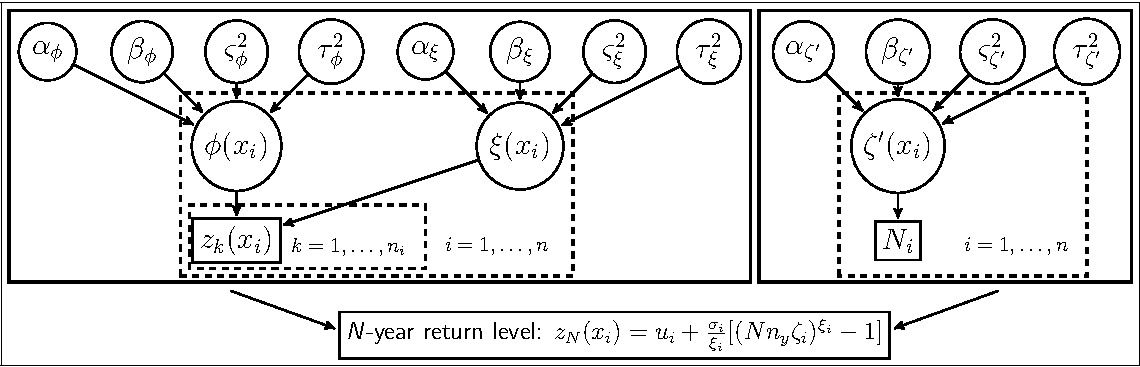
\includegraphics[width=1\linewidth]{waves-dag-cropped.pdf}
\caption{A directed acyclic graph (DAG) of the Bayesian spatial hierarchical models fitted to the wave data. On the left is the model for the excesses (using the GPD to model the data) and on the right is the model for the probability of an observation exceeding the threshold (using the Binomial distribution). The parameters of the distributions, modelled using Gaussian processes, are represented as circles in the middle layer, with the hyperparameters controlling these represented in the top layer. The data, modelled using the GPD for $z_k(x_i)$ and using a Binomial distribution for $N_i$, is represented in the bottom layer (in rectangles). Arrows run into nodes from their direct predecessors (often called parents). Given its parents, each node is independent of all other nodes in the graph except its descendants (often called children). Posterior estimates of the parameters' distributions can be used to form quantities of interest - typically return levels, as illustrated. Further details of each layer and the parameters involved may be found in the text.}
      \label{fig3:DAG3}
\end{figure}

\clearpage
\subsection*{Notation}

\begin{itemize}
\item $x_i$ Multivariate (bivariate or tri-variate) location values for location $i$, $i = 1,\ldots, n$. Write the matrix of all locations as just $x$
\item $z_k(x_i)$ $k$th observation at location $i$, $k = 1,\ldots,n_i$ where $n_i$ is the number of excesses at location $i$
\item $\sigma(x_i)$ Scale parameter for location $x_i$
\item $\phi(x_i) = \log(\sigma(x_i))$ The re-parameterised scale parameter
\item $\xi(x_i)$ Shape parameter for location $x_i$
%\item $z_k$ Sub-grid locations $k = 1, \ldots, m$. Together written as $z$
%\item $A, B$ Projection matrices of dimension $n \times m$
%\item $\phi^*, \xi^*$ Gaussian processes of $\phi$ and $\xi$ defined on sub-grid $z$
\item $\mu_\phi(x), \mu_\xi(x)$ Means for the Gaussian processes
\item $\Sigma, \Psi$ Covariance matrices for the Gaussian processes
\item $\tau^2_\phi, \tau^2_\xi$ Nugget parameters for the Gaussian processes
\item $\alpha_\phi, \alpha_\xi$ vectors of coefficients (including intercept) for Gaussian process means
\item $X_\phi, X_\xi$ Matrices of covariates (including column for intercept term) on the $x$ grid
%\item $\nu_\phi, \nu_\xi$ Matern smoothness parameters
\item $\beta_\phi, \beta_\xi$ Length scale scalars or matrices
\item $\varsigma^2_\phi, \varsigma^2_\xi$ Variance (partial sill) parameters for the Gaussian processes
\end{itemize}

\subsection*{Model outline} \label{3outline}

In hierarchical notation:
\begin{align*}
z_k(x_i) &\sim GPD(\sigma(x_i), \xi(x_i)) \\
\log (\sigma (x)) = \phi(x) &\sim MVN(\mu_\phi(x), \Sigma(x, x)) \\
%&= A(x, z) \Sigma^{-1}(z,z) \phi^*(z) \\
\xi (x) &\sim MVN(\mu_\xi(x), \Psi(x, x) )\\
%B(x, z) \Psi^{-1}(z,z) \xi^*(z) \\
%A(x_i, z_k) &= \varsigma_\phi^2 \frac{2^{1-\nu_\phi}}{\Gamma(\nu_\phi)}\Bigg(\sqrt{2\nu_\phi}\frac{\|x_i - z_k\|}{\beta_\phi}\Bigg)^{\nu_\phi} K_{\nu_\phi}\Bigg(\sqrt{2\nu_\phi}\frac{\|x_i - z_k\|}{\beta_\phi}\Bigg)\\
%B(x_i, z_k) &= \varsigma_\xi^2 \frac{2^{1-\nu_\xi}}{\Gamma(\nu_\xi)}\Bigg(\sqrt{2\nu_\xi}\frac{\|x_i - z_k\|}{\beta_\xi}\Bigg)^{\nu_\xi} K_{\nu_\xi}\Bigg(\sqrt{2\nu_\xi}\frac{\|x_i - z_k\|}{\beta_\xi}\Bigg)\\
%\phi^* &\sim MVN_m(\mu_\phi(z), \tau_\phi^2 I_m + \Sigma(z, z))\\
%\xi^* &\sim MVN_m(\mu_\xi(z), \tau_\xi^2 I_m + \Psi(z, z))\\
%\mu_\phi (z) &= Z_\phi \alpha_\phi \\
%\mu_\xi (z) &= Z_\xi \alpha_\xi \\
\mu_\phi(x) &= X_\phi \alpha_\phi \\
\mu_\xi(x) &= X_\xi \alpha_\xi \\
\Sigma(x_k, x_l) &= \varsigma_\phi^2 \exp \bigg(-\Big(\frac{d}{\beta_\phi}\Big)^2\bigg)  + \tau_\phi^2 \delta_{kl} \\
%\frac{2^{1-\nu_\phi}}{\Gamma(\nu_\phi)}\Bigg(\sqrt{2\nu_\phi}\frac{\|z_k - z_l\|}{\beta_\phi}\Bigg)^{\nu_\phi} K_{\nu_\phi}\Bigg(\sqrt{2\nu_\phi}\frac{\|z_k - z_l\|}{\beta_\phi}\Bigg)\\
\Psi(x_k, x_l) &= \varsigma_\xi^2 \exp \bigg(-\Big(\frac{d}{\beta_\xi}\Big)^2\bigg) + \tau_\xi^2 \delta_{kl} \\
%\frac{2^{1-\nu_\xi}}{\Gamma(\nu_\xi)}\Bigg(\sqrt{2\nu_\xi}\frac{\|z_k - z_l\|}{\beta_\xi}\Bigg)^{\nu_\xi} K_{\nu_\xi}\Bigg(\sqrt{2\nu_\xi}\frac{\|z_k - z_l\|}{\beta_\xi}\Bigg)
\end{align*}

$\delta_{kl}$ is the Kronecker delta function. In the above formulae for $\Sigma$ and $\Psi$, $\beta_\phi$ and $\beta_\xi$ are treated as scalars. When considered as matrices, where $d$ is the distance between two gridpoints, $(\sfrac{d}{\beta})^2$ is replaced by $d^T \beta^{-1} d$.
\\

Hyperparameter prior distributions (justifications for these values can be found in Section~\ref{sec:priors}):
\begin{align*}
\log(\varsigma^2_\phi), \log(\varsigma^2_\xi)&\sim N(0, 10) \\
\log(\tau^2_\phi), \log(\tau^2_\xi) &\sim N(0, 10) \\
\beta_\phi, \beta_\xi &\sim DU(0.001, 0.005, 0.01, 0.05, \dots , 100, 500, 1000)\\
%\nu_\phi, \nu_\xi &\sim DU(0.5, 2.5)\\
\alpha_{\phi,j} &\sim N(0, 50)\\
\alpha_{\xi,j} &\sim N(0, 50)\\
\end{align*}

%$\vec{\eta}_\phi$ and $\vec{\eta}_\xi$ are vectors of the appropriate length with all entries equal to 0. $H_\phi$ and $H_\xi$ are the relevant covariance matrices - to begin, these are diagonal matrices with 2 on the diagonal. The code is designed to allow the relationship between the coefficients to be modelled (if desired) by adjusting this covariance matrix.

\subsection*{Posterior distribution}

The full posterior distribution is:
\begin{align*}
p(\alpha_\phi, \alpha_\xi, \beta_\phi, \beta_\xi, \varsigma^2_\phi, \varsigma^2_\xi, \tau^2_\phi, \tau^2_\xi, \phi, \xi | x, z, X_\phi, X_\xi &) \propto \\
\left[ \prod_{i=1}^n \prod_{k=1}^{n_i} p(z_k(x_i) | \sigma(x_i)=\exp(\phi(x_i)), \xi(x_i)) \right] & \times \\
p(\phi(x) | \mu_\phi, \Sigma) p(\xi(x) | \mu_\xi, \Psi) & \times \\
p(\alpha_\phi) p(\alpha_\xi) p(\beta_\phi) p(\beta_\xi) & \times \\
p(\tau^2_\phi) p(\tau^2_\xi) p(\varsigma^2_\phi) p(\varsigma^2_\xi) &
\end{align*}

\subsection*{Conditional posterior distributions: Layer 2}

Updating the second layer of the DAG (parameters $\phi = \log(\sigma)$ and $\xi$): The conditional posterior distribution of $\phi$ is given by:

\begin{align*}
\pi(\phi | z, x, X_\phi, X_\xi, \alpha_\phi, \alpha_\xi, \beta_\phi, \beta_\xi, \varsigma^2_\phi, \varsigma^2_\xi, \tau^2_\phi, \tau^2_\xi, \xi) & \propto \\
\vspace{5 pt}
p(z | \phi, x, X_\phi, X_\xi, \alpha_\phi, \alpha_\xi, \beta_\phi, \beta_\xi, \varsigma^2_\phi, \varsigma^2_\xi, \tau^2_\phi, \tau^2_\xi, \xi) \hspace{3 pt} \times & \\
p(\phi | x, X_\phi, X_\xi, \alpha_\phi, \alpha_\xi, \beta_\phi, \beta_\xi, \varsigma^2_\phi, \varsigma^2_\xi, \tau^2_\phi, \tau^2_\xi, \xi) & \propto \\
p(z | \sigma, \xi)  p(\phi | \mu_\phi, \Sigma) &
\end{align*}

That is, the conditional posterior of $\phi$ is proportional to the product of the likelihood of the data $z$ given $\phi$ and all other parameters, and the prior probability density of $\phi$ given all of the other parameters. In the final line, most parameters have dropped out from the right-hand side, as the densities are independent of
these, given the remaining terms (see the DAG in Figure~\ref{fig3:DAG3} for this). Remember that $\phi = \log(\sigma)$ throughout this, where $\sigma$ is the scale parameter of the GPD, and note that $\mu_\phi$ and $\Sigma$ will have been calculated using the formulae in the model outline (above). \\

In briefer notation (to be used from now on):

\begin{align*}
\pi(\phi | \dots ) \propto & p(z | \sigma, \xi)  p(\phi | \mu_\phi, \Sigma) \\
= & \left[ \prod_{i=1}^n \prod_{k=1}^{n_i} p(z_k(x_i) | \sigma(x_i), \xi(x_i)) \right] p(\phi | \mu_\phi, \Sigma) \\
= & \left[ \prod_{i=1}^n \prod_{k=1}^{n_i} \frac{1}{\sigma(x_i)} \bigg( 1 + \xi(x_i) \frac{z_k(x_i)}{\sigma(x_i)} \bigg)^{-(\sfrac{1}{\xi(x_i)} + 1)} \right] \times \\
& \frac{1}{\sqrt{\det(2 \pi \Sigma)}} e^{-\frac{1}{2} (\phi - \mu_\phi)' \Sigma^{-1} (\phi - \mu_\phi) }
\end{align*}

Similarly:

\begin{align*}
\pi(\xi | \dots ) \propto & p(z | \phi, \xi)  p(\xi | \mu_\xi, \Psi) \\
= & \left[ \prod_{i=1}^n \prod_{k=1}^{n_i} p(z_k(x_i) | \sigma(x_i), \xi(x_i)) \right] p(\xi | \mu_\xi, \Psi) \\
= & \left[ \prod_{i=1}^n \prod_{k=1}^{n_i} \frac{1}{\sigma(x_i)} \bigg( 1 + \xi(x_i) \frac{z_k(x_i)}{\sigma(x_i)} \bigg)^{-(\sfrac{1}{\xi(x_i)} + 1)} \right] \times \\
& \frac{1}{\sqrt{\det(2 \pi \Psi)}} e^{-\frac{1}{2} (\xi - \mu_\xi)' \Psi^{-1} (\xi - \mu_\xi) }
\end{align*}

\subsubsection*{Metropolis-Hastings Markov chain Monte Carlo sampling}

In order to sample from these conditional posterior distributions, we use the Metropolis-Hastings Markov chain Monte Carlo (MCMC) algorithm. New samples are accepted or rejected at random according to the algorithm outlined below. \\

A new value of $\phi_i$ is suggested: $\phi^{'}_i$, where $i$ is a location on the grid, resulting in a new vector $\phi'$. \\

Suggested updates are drawn from a Normal distribution centred on the old value and with a variance of a manually set tuning parameter used to control the size of the proposed steps. \\

We calculate:

\begin{align*}
\rho(\phi_i, \phi^{'}_i) = \min \bigg (1, \frac{\pi(\phi^{'} | \dots ) q_t(\phi^{'}_i \to \phi_i)}{ \pi(\phi | \dots ) q_t(\phi_i \to \phi^{'}_i) } \bigg)
\end{align*}

where $\pi(\phi | \dots)$ is as defined above, and $q_t(a \to b)$ is the transition probability of proposing value $b$ given value $a$. Since updates are proposed using a Normal distribution, these transition probabilites above and below the line will always cancel, so the above simplifies to:

\begin{align*}
\rho(\phi_i, \phi^{'}_i) = \min \bigg (1, \frac{\pi(\phi^{'} | \dots ) }{ \pi(\phi | \dots ) } \bigg)
\end{align*}

Following this calculation, we always accept proposed value $\phi^{'}_i$ when $\rho(\phi_i, \phi^{'}_i)$ equals 1 and we reject accordingly when the ratio is smaller than 1 by simulating a random variable $u \sim U[0, 1]$ and accepting proposed value $\phi^{'}_i$ when $u\leq \rho(\phi_i, \phi^{'}_i)$. \\

Evaluating $\rho(\phi_i, \phi^{'}_i)$ typically involves products and quotients of many terms which may be close to 0. In order to work with something far more computationally stable, we use the property that $x = \exp(\log(x))$. Note also that since the vectors $\phi$ and $\phi^{'}$ differ in only one entry, the GPD calculations above and below will cancel for all other gridpoints apart from the one being updated, $i$. \\ 

Following these observations we need to evaluate:

\begin{align*}
\exp \bigg( & \log \bigg (\frac{\pi(\phi^{'} | \dots ) }{ \pi(\phi | \dots ) } \bigg) \bigg) \\
= \exp \big[ & \log(\pi(\phi^{'} | \dots )) - \log(\pi(\phi | \dots )) \big] \\
= \exp \Big[ & \log \Big( \Big[ \prod_{i=1}^n \prod_{k=1}^{n_i} p(z_k(x_i) | \sigma'(x_i), \xi(x_i)) \Big] p(\phi^{'} | \mu_\phi, \Sigma) \Big) - \\
& \log \Big( \Big[ \prod_{i=1}^n \prod_{k=1}^{n_i} p(z_k(x_i) | \sigma(x_i), \xi(x_i)) \Big] p(\phi | \mu_\phi, \Sigma) \Big) \Big] \\
= \exp \Big[ & \log \Big( \Big[ \prod_{k=1}^{n_i} p(z_k(x_i) | \sigma'(x_i), \xi(x_i)) \Big] p(\phi^{'} | \mu_\phi, \Sigma) \Big) - \\
& \log \Big( \Big[ \prod_{k=1}^{n_i} p(z_k(x_i) | \sigma(x_i), \xi(x_i)) \Big] p(\phi | \mu_\phi, \Sigma) \Big) \Big]
\end{align*}

Filling in the distribution details, this becomes:

\begin{align*}
 \exp \Bigg[ \log & \Big( \Big[ \prod_{k=1}^{n_i} \frac{1}{\sigma'(x_i)} \bigg( 1 + \xi(x_i) \frac{z_k(x_i)}{\sigma'(x_i)} \bigg)^{-(\sfrac{1}{\xi(x_i)} + 1)} \Big] \times \\
& \frac{1}{\sqrt{\det(2 \pi \Sigma)}} e^{-\frac{1}{2} (\phi^{'} - \mu_\phi)' \Sigma^{-1} (\phi^{'} - \mu_\phi) } \Big) \\
- \log & \Big( \Big[ \prod_{k=1}^{n_i} \frac{1}{\sigma(x_i)} \bigg( 1 + \xi(x_i) \frac{z_k(x_i)}{\sigma(x_i)} \bigg)^{-(\sfrac{1}{\xi(x_i)} + 1)} \Big] \times \\
& \frac{1}{\sqrt{\det(2 \pi \Sigma)}} e^{-\frac{1}{2} (\phi - \mu_\phi)' \Sigma^{-1} (\phi - \mu_\phi) } \Big) \Bigg] \\
= \exp \Bigg[ \sum_{k=1}^{n_i} \log & \Big( \Big[ \frac{1}{\sigma'(x_i)} \bigg( 1 + \xi(x_i) \frac{z_k(x_i)}{\sigma'(x_i)} \bigg)^{-(\sfrac{1}{\xi(x_i)} + 1)} \Big] \Big) + \\
& \log \Bigg( \frac{1}{\sqrt{\det(2 \pi \Sigma)}} \Bigg) -\frac{1}{2} (\phi^{'} - \mu_\phi)' \Sigma^{-1} (\phi^{'} - \mu_\phi) \\
- \sum_{k=1}^{n_i} \log & \Big( \Big[  \frac{1}{\sigma(x_i)} \bigg( 1 + \xi(x_i) \frac{z_k(x_i)}{\sigma(x_i)} \bigg)^{-(\sfrac{1}{\xi(x_i)} + 1)} \Big] \Big) - \\
& \log \Bigg( \frac{1}{\sqrt{\det(2 \pi \Sigma)}} \Bigg) +\frac{1}{2} (\phi - \mu_\phi)' \Sigma^{-1} (\phi - \mu_\phi) \Bigg] \\
= \exp \Bigg[ \sum_{k=1}^{n_i} \log & \Big( \Big[ \frac{1}{\sigma'(x_i)} \bigg( 1 + \xi(x_i) \frac{z_k(x_i)}{\sigma'(x_i)} \bigg)^{-(\sfrac{1}{\xi(x_i)} + 1)} \Big] \Big) - \\
& \frac{1}{2} (\phi^{'} - \mu_\phi)' \Sigma^{-1} (\phi^{'} - \mu_\phi) - \\
\sum_{k=1}^{n_i} \log & \Big( \Big[  \frac{1}{\sigma(x_i)} \bigg( 1 + \xi(x_i) \frac{z_k(x_i)}{\sigma(x_i)} \bigg)^{-(\sfrac{1}{\xi(x_i)} + 1)} \Big] \Big) + \\
& \frac{1}{2} (\phi - \mu_\phi)' \Sigma^{-1} (\phi - \mu_\phi) \Bigg]
\end{align*}

The common term $\log(\sfrac{1}{\sqrt{\det(2 \pi \Sigma)}})$ in both numerator and denominator above dropped out as it will be equal in both (it has no dependence on $\phi$). \\

The GPD can clearly be simplified further using the properties of logs. Just taking one of the functions on its own for clarity:

\begin{align*}
\sum_{k=1}^{n_i} \log & \Bigg( \Bigg[ \frac{1}{\sigma'(x_i)} \bigg( 1 + \xi(x_i) \frac{z_k(x_i)}{\sigma'(x_i)} \bigg)^{-(\sfrac{1}{\xi(x_i)} + 1)} \Bigg] \Bigg) = \\
\sum_{k=1}^{n_i} \Bigg[ \log & \Big( \frac{1}{\sigma'(x_i)} \Big) + \log \bigg( 1 + \xi(x_i) \frac{z_k(x_i)}{\sigma'(x_i)} \bigg)^{-(\sfrac{1}{\xi(x_i)} + 1)} \Bigg] = \\
\sum_{k=1}^{n_i} \Bigg[ - \log & (\sigma'(x_i)) - \bigg( \frac{1}{\xi(x_i)} + 1 \bigg) \log \bigg( 1 + \xi(x_i) \frac{z_k(x_i)}{\sigma'(x_i)} \bigg) \Bigg]
\end{align*}

Using this form, the full term we need to evaluate in order to update $\phi$ is:

\begin{align}
= \exp \Bigg[ \sum_{k=1}^{n_i} \bigg[ - \log (\sigma'(x_i)) - \bigg( \frac{1}{\xi(x_i)} + 1 \bigg) \log \bigg( 1 + \xi(x_i) \frac{z_k(x_i)}{\sigma'(x_i)} \bigg) \bigg] & - \nonumber \\
\frac{1}{2} (\phi^{'} - \mu_\phi)' \Sigma^{-1} (\phi^{'} - \mu_\phi) & - \nonumber \\
\sum_{k=1}^{n_i} \bigg[ - \log (\sigma(x_i)) - \bigg( \frac{1}{\xi(x_i)} + 1 \bigg) \log \bigg( 1 + \xi(x_i) \frac{z_k(x_i)}{\sigma(x_i)} \bigg) \bigg] & + \nonumber \\
\frac{1}{2} (\phi - \mu_\phi)' \Sigma^{-1} (\phi - \mu_\phi) \Bigg] & \label{3eq:1a}
\end{align}

Similar reasoning leads to the update for $\xi$. We need to evaluate:

\begin{align*}
\rho(\xi_i, \xi^{'}_i) = \min \bigg (1, \frac{\pi(\xi^{'} | \dots ) q_t(\xi^{'}_i \to \xi_i)}{ \pi(\xi | \dots ) q_t(\xi_i \to \xi^{'}_i) } \bigg)
\end{align*}

The full term we need to evaluate is:

\begin{align}
= \exp \Bigg[ \sum_{k=1}^{n_i} \bigg[ - \log (\sigma(x_i)) - \bigg( \frac{1}{\xi'(x_i)} + 1 \bigg) \log \bigg( 1 + \xi'(x_i) \frac{z_k(x_i)}{\sigma(x_i)} \bigg) \bigg] & -\nonumber \\
\frac{1}{2} (\xi' - \mu_\xi)' \Psi^{-1} (\xi' - \mu_\xi) & - \nonumber \\
\sum_{k=1}^{n_i} \bigg[ - \log (\sigma(x_i)) - \bigg( \frac{1}{\xi(x_i)} + 1 \bigg) \log \bigg( 1 + \xi(x_i) \frac{z_k(x_i)}{\sigma(x_i)} \bigg) \bigg] & +\nonumber \\
\frac{1}{2} (\xi - \mu_\xi)' \Psi^{-1} (\xi - \mu_\xi) \Bigg] & \label{3eq:1b}
\end{align}


\subsection*{Conditional posterior distributions: Layer 3}

\subsubsection*{\pmb{$\alpha$}}

Updating the third layer of the DAG (that is, all hyperparameters) starting with $\alpha_\phi$:

\begin{align*}
\pi(\alpha_\phi | z, \dots ) \propto & p(z | \alpha_\phi, \dots ) p(\alpha_\phi | \dots) \\
\propto & p(z | \sigma, \xi)  p(\phi | \mu_\phi, \Sigma) p(\alpha_\phi) \\
\propto & p(\phi | \mu_\phi, \Sigma) p(\alpha_\phi)
\end{align*}

Essentially the GPD component is independent of $\alpha_\phi$ once the other parameters are known, and so can be absorbed into the constant of proportionality. What we're left with is the $MVN$ piece (since $\alpha_\phi$ features in the calculation of $\mu_\phi$) and the prior on $\alpha_\phi$. \\

Then we have:

\begin{align*}
\pi(\alpha_\phi | \dots ) \propto & p(\phi | \mu_\phi, \Sigma) p(\alpha_\phi) \\
\propto & \frac{1}{\sqrt{\det(2 \pi \Sigma)}} e^{-\frac{1}{2} (\phi - \mu_\phi)' \Sigma^{-1} (\phi - \mu_\phi) } \times \\
& \frac{1}{\sqrt{2 \pi s^2}} e^{-\frac{(\alpha_\phi - m)^2}{2 s^2}}
\end{align*}

where $m$ is the prior mean and $s^2$ is the prior variance. In a slight abuse of notation in the final line above, $\alpha_\phi$ is a scalar, the single element which is being updated from the vector $\alpha_\phi$.
\\

Similarly:

\begin{align*}
\pi(\alpha_\xi | \dots ) \propto & p(\xi | \mu_\xi, \Psi) p(\alpha_\xi) \\
\propto & \frac{1}{\sqrt{\det(2 \pi \Psi)}} e^{-\frac{1}{2} (\xi - \mu_\xi)' \Psi^{-1} (\xi - \mu_\xi) } \times \\
& \frac{1}{\sqrt{2 \pi s^2}} e^{-\frac{(\alpha_\xi - m)^2}{2 s^2}}
\end{align*}

where $m$ is the prior mean and $s^2$ is the prior variance, and a similar slight abuse of notation applies in the final line for $\alpha_\xi$.
\\

As with the parameters $\phi$ and $\xi$, updates for $\alpha_\phi$ are suggested element-wise: $\alpha_{\phi,\kappa} \to \alpha'_{\phi,\kappa}$, where the index $\kappa$ runs over the vector of coefficients. The ratio $\rho(\alpha_{\phi,\kappa}, \alpha'_{\phi,\kappa})$ is then calculated. Similar manipulations to those used in the previous section lead to the following calculation needed to update $\alpha_\phi$:

\begin{align}
\exp \Big[ - \frac{1}{2} & \log(\det(2 \pi \Sigma)) -\frac{1}{2} (\phi - \mu'_\phi)' \Sigma^{-1} (\phi - \mu'_\phi) \nonumber \\
& - \frac{1}{2} \log(2 \pi s^2) -\frac{(\alpha'_{\phi,\kappa} - m)^2}{2 s^2} \nonumber \\
& + \frac{1}{2} \log(\det(2 \pi \Sigma)) + \frac{1}{2} (\phi - \mu_\phi)' \Sigma^{-1} (\phi - \mu_\phi) \nonumber \\
& + \frac{1}{2} \log(2 \pi s^2) + \frac{(\alpha_{\phi,\kappa} - m)^2}{2 s^2} \Big] = \nonumber \\
\exp \Big[ -\frac{1}{2} & (\phi - \mu'_\phi)' \Sigma^{-1} (\phi - \mu'_\phi) -\frac{(\alpha'_{\phi,\kappa} - m)^2}{2 s^2} \nonumber \\
& + \frac{1}{2} (\phi - \mu_\phi)' \Sigma^{-1} (\phi - \mu_\phi) +  \frac{(\alpha_{\phi,\kappa} - m)^2}{2 s^2}
\Big] \label{3eq:2a1}
\end{align}

And for $\alpha_\xi$:

\begin{align}
\exp \Big[ -\frac{1}{2} & (\xi - \mu'_\xi)' \Psi^{-1} (\xi - \mu'_\xi) -\frac{(\alpha'_{\xi,\kappa} - m)^2}{2 s^2} \nonumber \\
& + \frac{1}{2} (\xi - \mu_\xi)' \Psi^{-1} (\xi - \mu_\xi) + \frac{(\alpha_{\xi,\kappa} - m)^2}{2 s^2}
\Big] \label{3eq:2a2}
\end{align}

Updates for the other hyperparameters are similar. The matrices $\Sigma$ and $\Psi$ will change with any change in $\beta, \varsigma^2$ or $\tau^2$. The remaining hyperparameters either have a discrete update (in which case the prior probability will be $\sfrac{1}{\#discrete.values}$ and will cancel above and below the line, or have a univariate Normal prior on them (or their log). \\

\subsubsection*{\pmb{$\beta$}}

For $\beta_\phi$ we have:

\begin{align*}
\pi(\beta_\phi | \dots ) \propto & p(\phi | \mu_\phi, \Sigma) p(\beta_\phi)
\end{align*}

Since $\beta_\phi$ has a discrete prior, to update $\beta_\phi$ we need to evaluate:

\begin{align}
\exp \Big[ & - \frac{1}{2}  \log(\det(2 \pi \Sigma')) -\frac{1}{2} (\phi - \mu_\phi)' \Sigma'^{-1} (\phi - \mu_\phi) \nonumber \\
& + \frac{1}{2} \log(\det(2 \pi \Sigma)) + \frac{1}{2} (\phi - \mu_\phi)' \Sigma^{-1} (\phi - \mu_\phi) \Big] \label{3eq:2b1}
\end{align}

where $\Sigma'$ has been formed using $\beta'_\phi$, the new proposal value or matrix. \\

Then for $\beta_\xi$ we have:

\begin{align*}
\pi(\beta_\xi | \dots ) \propto & p(\xi | \mu_\xi, \Psi) p(\beta_\xi)
\end{align*}

To update $\beta_\xi$ we need to evaluate:

\begin{align}
\exp \Big[ & -\frac{1}{2} \log(\det(2 \pi \Psi')) -\frac{1}{2} (\xi - \mu_\xi)' \Psi'^{-1} (\xi - \mu_\xi) \nonumber \\
& + \frac{1}{2} \log(\det(2 \pi \Psi))+ \frac{1}{2} (\xi - \mu_\xi)' \Psi^{-1} (\xi - \mu_\xi) \Big] \label{3eq:2b2}
\end{align}

where $\Psi'$ has been formed using $\beta'_\xi$, the new proposal value or matrix. \\

%\subsubsection*{\pmb{$\nu$}}
%
%$\nu_\phi$ also has a discrete update and so will look identical to the update for $\beta_\phi$. It has conditional posterior distribution of:
%
%\begin{align*}
%\pi(\nu_\phi | \dots ) \propto & p(\phi^* | \mu_\phi, \tau^2_\phi, \Sigma) p(\nu_\phi)
%\end{align*}
%
%We need to evaluate:
%
%\begin{align}
%\exp \Big[ & - \frac{1}{2}  \log(\det(2 \pi (\Sigma' + \tau^2_\phi I_m))) -\frac{1}{2} (\phi^* - \mu_\phi)' (\Sigma' + \tau^2_\phi I_m)^{-1} (\phi^* - \mu_\phi) \nonumber \\
%& + \frac{1}{2} \log(\det(2 \pi (\Sigma + \tau^2_\phi I_m))) + \frac{1}{2} (\phi^* - \mu_\phi)' (\Sigma + \tau^2_\phi I_m)^{-1} (\phi^* - \mu_\phi) \Big] \label{3eq:2n1}
%\end{align}
%
%where $\Sigma'$ has been formed using $\nu'_\phi$, the new proposal value. \\
%
%In order to update $\nu_\xi$ we have:
%
%\begin{align*}
%\pi(\nu_\xi | \dots ) \propto & p(\xi^* | \mu_\xi, \tau^2_\xi, \Psi) p(\nu_\xi)
%\end{align*}
%
%We therefore need to evaluate:
%
%\begin{align}
%\exp \Big[ & -\frac{1}{2} \log(\det(2 \pi (\Psi' + \tau^2_\xi I_m))) -\frac{1}{2} (\xi^* - \mu_\xi)' (\Psi' + \tau^2_\xi I_m)^{-1} (\xi^* - \mu_\xi) \nonumber \\
%& + \frac{1}{2} \log(\det(2 \pi (\Psi + \tau^2_\xi I_m)))+ \frac{1}{2} (\xi^* - \mu_\xi)' (\Psi + \tau^2_\xi I_m)^{-1} (\xi^* - \mu_\xi) \Big] \label{3eq:2n2}
%\end{align}
%
%where $\Psi'$ has been formed using $\nu'_\xi$, the new proposal value. \\

\subsubsection*{\pmb{$\varsigma^2$}}

$\varsigma^2_\phi$ has a conditional posterior distribution of:

\begin{align*}
\pi(\varsigma^2_\phi | \dots ) \propto & p(\phi | \mu_\phi, \Sigma) p(\varsigma^2_\phi)
\end{align*}

The prior distribution of the log of $\varsigma^2_\phi$ is a univariate Normal. So to update $\varsigma^2_\phi$ we need to evaluate:

\begin{align}
\exp \Bigg[ - \frac{1}{2}  & \log(\det(2 \pi \Sigma')) - \nonumber \\
\frac{1}{2} &  (\phi - \mu_\phi)' \Sigma'^{-1} (\phi - \mu_\phi) -
 \frac{(\log(\varsigma^{2'}_\phi) - m)^2}{2 s^2} + \nonumber \\
\frac{1}{2}  & \log(\det(2 \pi \Sigma)) + \nonumber \\
\frac{1}{2} & (\phi - \mu_\phi)' \Sigma^{-1} (\phi - \mu_\phi) + \frac{(\log(\varsigma^2_\phi) - m)^2}{2 s^2} \Bigg] \label{3eq:2vs1}
\end{align}

where $\Sigma'$ has been formed using $\varsigma^{2'}_\phi$, the new proposal value, and $m$ and $s$ are the prior mean and standard deviation repectively. \\

$\varsigma^2_\xi$ has a conditional posterior distribution of:

\begin{align*}
\pi(\varsigma^2_\xi | \dots ) \propto & p(\xi | \mu_\xi, \Psi) p(\varsigma^2_\xi)
\end{align*}

To update $\varsigma^2_\xi$ we need to evaluate:

\begin{align}
\exp \Bigg[ -\frac{1}{2} & \log(\det(2 \pi \Psi')) - \nonumber \\
\frac{1}{2} & (\xi - \mu_\xi)' \Psi'^{-1} (\xi - \mu_\xi) - \frac{(\log(\varsigma^{2'}_\xi) - m)^2}{2 s^2} + \nonumber \\
\frac{1}{2} & \log(\det(2 \pi \Psi)) +\nonumber \\
\frac{1}{2} & (\xi - \mu_\xi)' \Psi^{-1} (\xi - \mu_\xi) + \frac{(\log(\varsigma^2_\xi) - m)^2}{2 s^2} \Bigg] \label{3eq:2vs2}
\end{align}

where $\Psi'$ has been formed using $\varsigma^{2'}_\xi$, the new proposal value, and $m$ and $s$ are the prior mean and standard deviation repectively. \\

\subsubsection*{\pmb{$\tau^2$}}

$\tau^2_\phi$ has a conditional posterior distribution of:

\begin{align*}
\pi(\tau^2_\phi | \dots ) \propto & p(\phi | \mu_\phi, \Sigma) p(\tau^2_\phi)
\end{align*}

The prior distribution of the log of $\tau^2_\phi$ is a univariate Normal. So to update $\tau^2_\phi$ we need to evaluate:

\begin{align}
\exp \Bigg[ - \frac{1}{2} & \log(\det(2 \pi \Sigma')) - \nonumber \\
\frac{1}{2} & (\phi - \mu_\phi)' \Sigma'^{-1} (\phi - \mu_\phi) - \frac{(\log(\tau^{2'}_\phi) - m)^2}{2 s^2} + \nonumber \\
\frac{1}{2} & \log(\det(2 \pi \Sigma)) + \nonumber \\
\frac{1}{2} & (\phi - \mu_\phi)' \Sigma^{-1} (\phi - \mu_\phi) + \frac{(\log(\tau^2_\phi) - m)^2}{2 s^2} \Bigg] \label{3eq:2t1}
\end{align}

where $\Sigma'$ has been formed using $\tau^{2'}_\phi$, the new proposal value, and $m$ and $s$ are the prior mean and standard deviation repectively. \\

$\tau^2_\xi$ has a conditional posterior distribution of:

\begin{align*}
\pi(\tau^2_\xi | \dots ) \propto & p(\xi | \mu_\xi, \Psi) p(\tau^2_\xi)
\end{align*}

To update $\tau^2_\xi$ we need to evaluate:

\begin{align}
\exp \Bigg[ -\frac{1}{2} & \log(\det(2 \pi \Psi')) - \nonumber \\
\frac{1}{2} & (\xi - \mu_\xi)' \Psi'^{-1} (\xi - \mu_\xi) - \frac{(\log(\tau^{2'}_\xi) - m)^2}{2 s^2} + \nonumber \\
\frac{1}{2} & \log(\det(2 \pi \Psi)) +\nonumber \\
\frac{1}{2} & (\xi - \mu_\xi)' \Psi^{-1} (\xi - \mu_\xi) + \frac{(\log(\tau^2_\xi) - m)^2}{2 s^2} \Bigg] \label{3eq:2t2}
\end{align}

where $\Psi'$ has been formed using $\tau^{2'}_\xi$, the new proposal value, , and $m$ and $s$ are the prior mean and standard deviation repectively.

\end{document}
